\subsubsection{Detectors}\label{sec:detectors}
Information and status of connected detectors are displayed in this tab.
\begin{figure}[H]
    \centering
    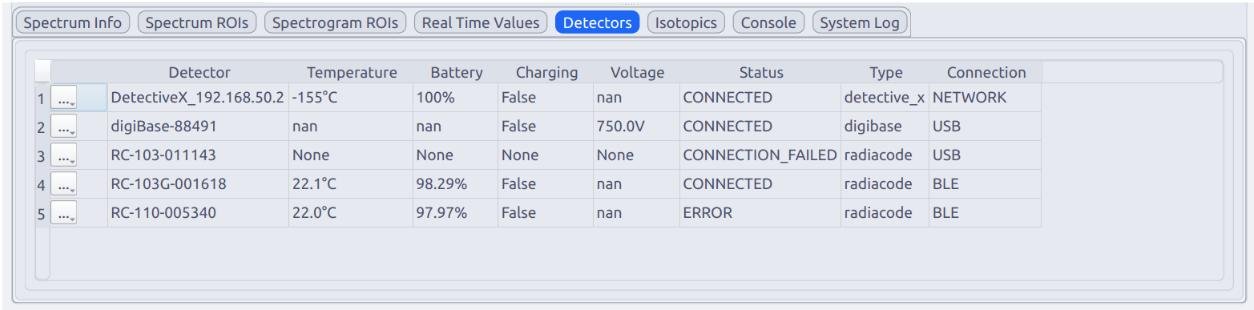
\includegraphics[width = .9\linewidth]{images/interface/detectors_tab.jpg}
    \caption{List of connected detectors. An entry can not be removed, if a detector is disconnected it is listed as \texttt{STOPPED}.}
    \label{fig:detector_tab}
\end{figure}

\begin{table}[H]
    \centering
    \caption{Description of the columns in the Detectors tab}
    \label{tab:detectors_tab}
    \begin{tabular}{p{.3\textwidth}p{.64\textwidth}}
    \toprule
    \textbf{Column} & \textbf{Description} \\ \midrule
        Column 0 & Options button marked with '...', see \autoref{tab:detectors_options_button}. \\
        Detector & The name of the detector. \\
        Temperature & The temperature reading from the detector in $^\circ$C. Most detectors report the ambient temperature but some, like the Detective X, report the cooled crystal temperature, as seen in \autoref{fig:detector_tab}. \\
        Battery & The current battery level in \%. \\
        Charging & Indicate if the detector is connected to a power source. \\
        Voltage & The actual voltage reported of the detector in V. \\
        Status & Detector state reported as one of the following options: 
        \begin{itemize}
            \item \texttt{UNINITIALIZED} - Detector client created but not started.
            \item \texttt{CONNECTING} - The detector is starting.
            \item \texttt{CONNECTED} - The detector is connected and running. Default for normal detector function.
            \item \texttt{CONNECTION\_FAILED} - Detector start failed. Check System Log.
            \item \texttt{CONNECTION\_LOST} - Connection was lost after a successful start. Not universally implemented.
            \item \texttt{STOPPING} - The detector has received and acknowledged the command to stop.
            \item \texttt{STOPPED} - The detector has successfully stopped.
            \item \texttt{ERROR} - An error occurred while connected and the detector is no longer functioning as expected.
        \end{itemize} \\
        Type & Type of detector by the name defined in the detector client. \\
        Connection & How the detector is connected. Can be \texttt{BLE, USB} or \texttt{NETWORK}. \\
    \bottomrule
    \end{tabular}
\end{table}

\begin{table}[H]
    \centering
    \caption{Description of the options menu in the detector tab, opened with the button marked '...' in the table.}
    \label{tab:detectors_options_button}
    \begin{tabular}{p{.3\textwidth}p{.64\textwidth}}
    \toprule
    \textbf{Field} & \textbf{Description} \\ \midrule
        Disconnect & Sends a stop signal to the detector. \\
        Reset Spectrum & Signals to the selected detector to clear its spectrum. \\
        Start Acquisition & Signals to the selected detector to start spectrum acquisition. \\
        Stop Acquisition & Signals to the selected detector to stop spectrum acquisition. \\
        Make Instrument & Shortcut for creating a \textit{Unique Instrument} for the detector based on a \texttt{Generic Instrument} and save the current calibration of the connected spectrum. Useful for detectors that do not Library their own energy calibration. \\
        Settings & Opens the detector settings dialog, see \autoref{fig:detector_settings_calibration} and \autoref{fig:detector_settings_mca}. \\
    \bottomrule
    \end{tabular}
\end{table}

\begin{figure}[H]
    \centering
    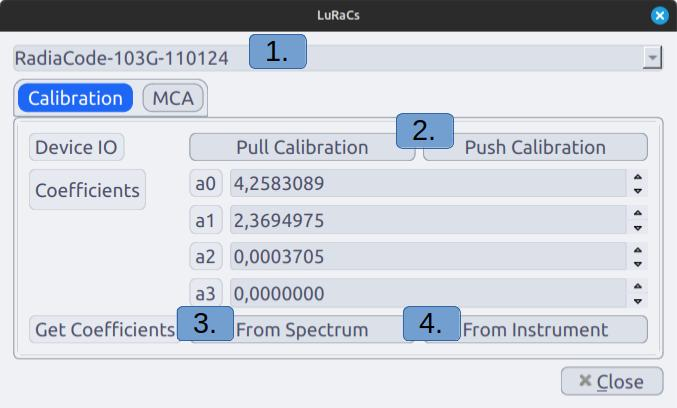
\includegraphics[width = .6\linewidth]{images/interface/detector_settings_calibration.jpg}
    \caption{Detector settings dialog showing the options for setting device calibration.}
    \label{fig:detector_settings_calibration}
    \begin{flushleft}
        \begin{enumerate}
            \item Unique Instrument from the library to pull settings from.
            \item Interact with the detector. \texttt{Pull Calibration} will request a calibration from the detector set in the coefficients buffer, not possible for all detectors. \texttt{Push Calibration} will attempt to set the calibration of the detector, not possible for all detectors.
            \item Pull the calibration coefficients from the spectrum connected to the detector and set in the coefficients buffer.
            \item Pull the calibration coefficients from the instrument set in (1.) and set in the coefficients buffer
        \end{enumerate}
    \end{flushleft}
\end{figure}

\begin{figure}[H]
    \centering
    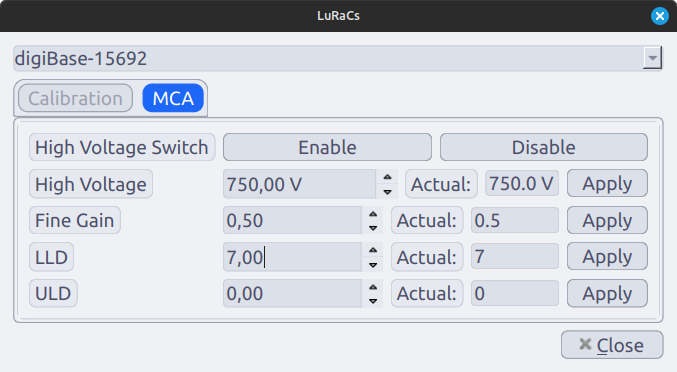
\includegraphics[width = .6\linewidth]{images/interface/detector_settings_mca.png}
    \caption{Detector settings dialog showing the options for MCA settings. The first column of spinboxes show the requested setting and the second row shows the actual value reported by the instrument. \texttt{Apply} attempts to set the given value to the detector.}
    \label{fig:detector_settings_mca}
    \begin{tabular}{ll}
    LLD & Lower Level Discriminator \\
    ULD & Upper Lever Discriminator
    \end{tabular}
  
\end{figure}